\documentclass[usletter]{article}
\usepackage{graphicx}
\usepackage{amsfonts}
\usepackage{amsthm}
\usepackage{amsmath}
\usepackage{scribe}
\usepackage[margin=1.5in]{geometry}
\usepackage{algorithm}
\usepackage{algorithmicx}
\usepackage[noend]{algpseudocode}

\begin{document}

\makeheader{Minsheng Zhang}                              % your name
           {February 8, 2015}                          % lecture date
           {5}                                       % lecture number
           {Transformation and LP}  % lecture title

\noindent
During this week, in the first lecture we talked about how to optimize the solution for vetex cover problem. Then for the other two lectures we discussed about linear programming problems and the primal dual method. 

\section{Vetex Cover}
Recall that a vertex cover is a set of k vertices such that each edge in a graph is adjacent to at least one vertex in the set. The problem of finding a minimum vertex cover is a classical optimization problem in computer science and is a typical example of an NP-hard optimization problem that has an approximation algorithm.  We solve the problem by converting it to the a decision problem. Using the decision version, we have made the problem parametrization.

Formally, a vertex-cover of an undirected graph $G=(V, E)$ is a subset V′ of V such that if edge (u, v) is an edge of G, then u is in V′, or v is in V′, or both. The set V′ is said to $"cover"$ the edges of G. The Figure~\ref{fig:example} shows examples of vertex covers in two graphs (and the set V' is marked with red).
\begin{figure}[bht]
\begin{center}
     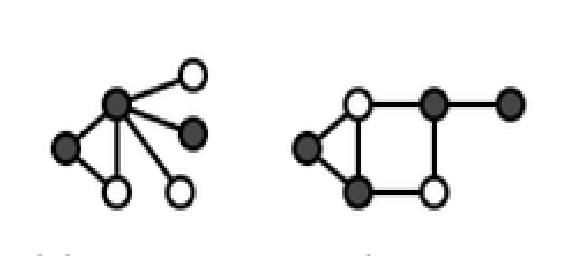
\includegraphics[width=2.0in]{figures/vc1}
\caption{\label{fig:example}Vetex Cover Example}
\end{center}
\end{figure}

A minimum vertex cover is a vertex cover of smallest possible size. The vertex cover number is the size of a minimum vertex cover. The Figure~\ref{fig:solution} shows examples of minimum vertex covers in the previous graphs.
\begin{figure}[bht]
\begin{center}
     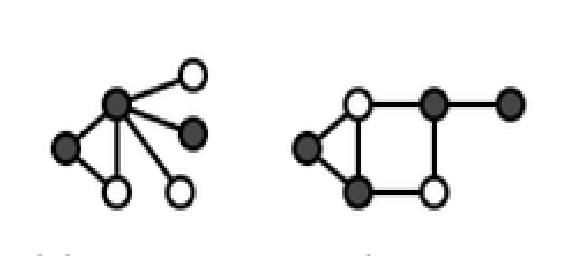
\includegraphics[width=2.0in]{figures/vc1}
\caption{\label{fig:solution}Vetex Cover Example}
\end{center}
\end{figure}

The minimum vertex cover problem is: 
\begin{enumerate}
	\item INSTANCE: Graph G
	\item OUTPUT: Smallest number k such that G has a vertex cover of size k.
\end{enumerate}


The decision version of the problem:
\begin{enumerate}
	\item INSTANCE: Graph G and positive integer k.
	\item QUESTION: Does G have a vertex cover of size at most k?
\end{enumerate}

\begin{algorithm}
\caption{VC}
\begin{algorithmic}[1]
\Procedure{VC}{G, k}
\If {k == 0 or E is empty} 
	\State \Return $|E|$ == 0
\EndIf
\State pick an edge (u,v) from E
\State $G_{1}$ = G - \{u\}
\State $G_{2}$ = G - \{v\}
\State \Return \Call{VC}{$G_{1}$, k-1} or \Call{VC}{$G_{2}$, k-1}
\EndProcedure
\end{algorithmic}
\end{algorithm}

In this problem, K is the size in the decision problem, n is the size of the graph. We assume the algorithm complexity is $T(n)$, then $T(n, k)$ would be equal to  $2*T(n-1, k-1)+n$. Using mathematics induction, the result would be $O(2^{k}n)$.

After that, we try to improve the algorithm a little bit and make the time complexity of the problem only be relevant to the size of K.

\begin{algorithm}
\caption{VC2}
\begin{algorithmic}[1]
\Procedure{VC2}{G, k}
\State $m=vetices with degree larger than k$
\If {$m > k$} 
	\State \Return False
\EndIf
\State G' = Removing m vertices with degree $> k$ and = 0 in G. 
\State \Return \Call{VC}{G', k-m} 
\EndProcedure
\end{algorithmic}
\end{algorithm}
The reason here why we can reduce the size to k-m is: 
\begin{enumerate}
	\item If the vertex is not in the vertex cover solution, then all its neighbor should be in it. As this node has at least k degree, then it has at least k neighbors, if so, it should return false.
	\item This vertex must be in the vertex cover solution, if the desicion problem for K is true. So we can remove these m nodes as they must be in the solution.
\end{enumerate}

So we can subsitute the complexity with n to K. First we have at most (k-m) vertices. Then maximum edges is (k-m)*k. Then we have at most 2*(k-m)*k vertices which is less than $2k^2$. So the time complexity is $O(2^{k}*k^{2})$ 

\section{Convex Hull}
Then we discussed the problem convex hull.  The convex hull of a set X of points in the Euclidean plane or Euclidean space is the smallest convex set that contains X. For instance, when X is a bounded subset of the plane, the convex hull may be visualized as the shape formed by a rubber band stretched around X.
Figure~\ref{fig:convex-hull} shows the result of a convex hall problem. The result for the problem will be sorted using the x-plane value, or rotated sorted.

\begin{figure}[bht]
\begin{center}
     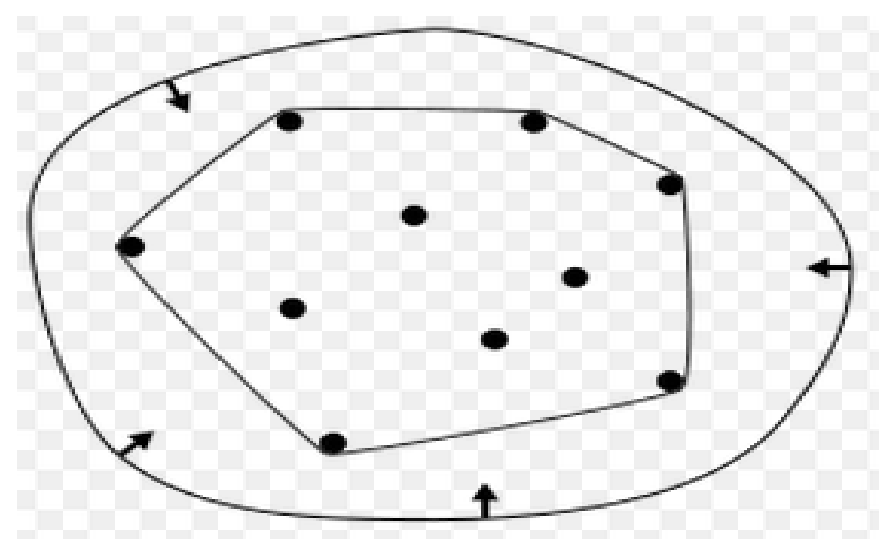
\includegraphics[width=2.0in]{figures/ch}
\caption{\label{fig:convex-hull}Convex Hull example}
\end{center}
\end{figure}

We use this example to show that we can use transformation to prove the complexity of an algorithm or we can say that we have got the best time complexity of a problem. In computational geometry, a number of algorithms are known for computing the convex hull with the time complexity at least $O(nlogn)$. We can use transformation to prove that this is the best we can get.

We will transform the sort problem into convex hull problem. Assume we have a list of numbers. We want to sort all these problems. We can map all the points into a 2D plane using the formular $y=x^2$, then we can consider it as a convex hull problem in Figure~\ref{fig:convex-hull}.  After getting the result of the convex hull, we can get the result for sort problem as the result of the convex hull will be sorted by the x-plane or rotated sorted. If the result is rotated sorted, we can easily get the sort results using $O(n)$ time. So if we can solve the convex hull problem in $O(n)$, we can solve the sort problem using $O(n)$ too as the transformation from sorting to convex hull is $O(n)$.  But we can illustrate that the time complexity of sorting is at least $O(nlogn)$, then we can say that we have got solution with the best performace for convex hull.
\begin{figure}[bht]
\begin{center}
     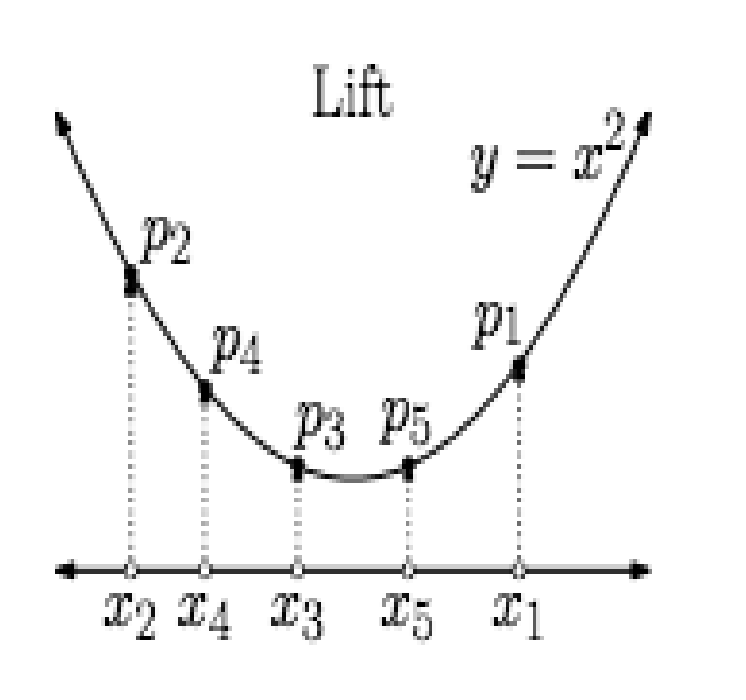
\includegraphics[width=2.0in]{figures/convex-hull}
\caption{\label{fig:convex-hull}Convex Hull example}
\end{center}
\end{figure}

Assume we have three numbers a, b, c. To sort these numbers, we can make a decision tree for the problem in Figure~\ref{fig:decision-tree}.

\begin{figure}[bht]
\begin{center}
     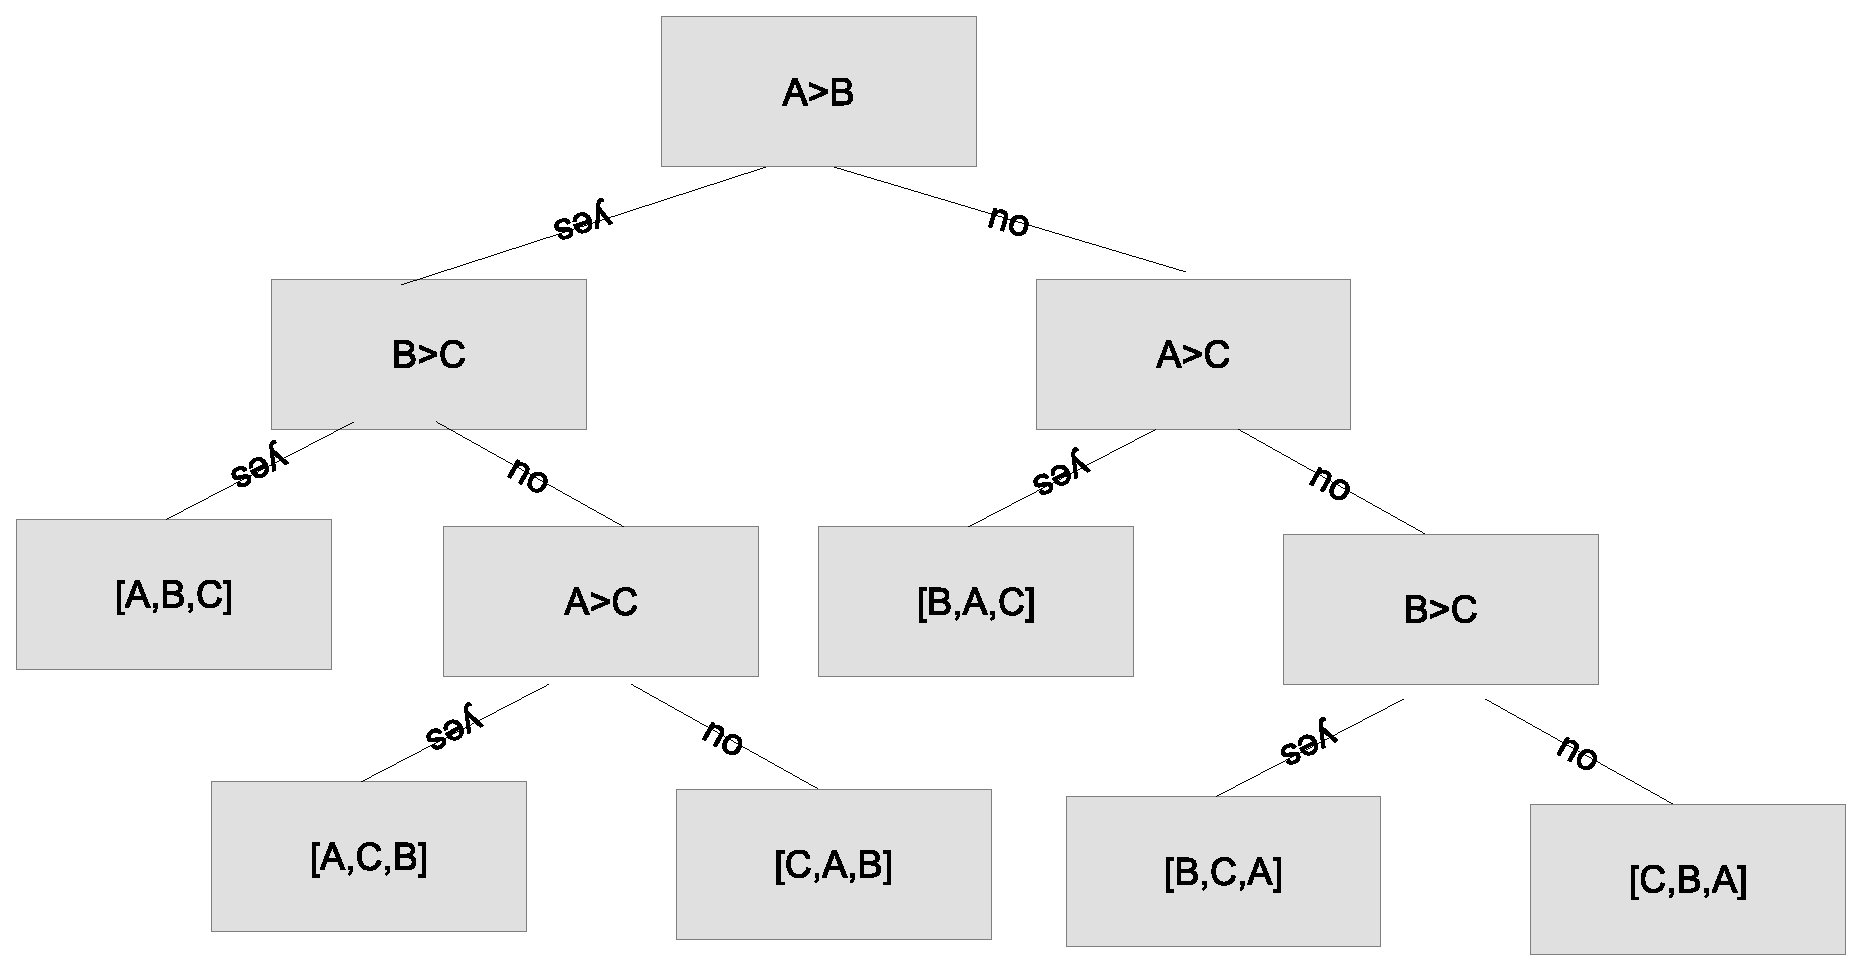
\includegraphics[width=4.0in]{figures/decision-tree}
\caption{\label{fig:decision-tree}Decision Tree for sort}
\end{center}
\end{figure}

Furthermore, it is the height of the binary decision tree that determines the worst-case running time of the algorithm. In general, the size and shape of the decision tree depends on the sorting algorithm and the number of items to be sorted. 

Given an input sequence of n items to be sorted, every binary decision tree that correctly sorts the input sequence must have at least $n!$ leaves--one for each permutation of the input. So the height of the binary tree is at least:


Since the height of the decision tree is  $O(nlogn)$, the number of comparisons done by any sorting algorithm that sorts using only binary comparisons is  $O(nlogn)$. Assuming each comparison can be done in constant time, the running time of any such sorting algorithm is  $O(nlogn)$. 

As we have got that the sort problem should run at least $O(nlogn)$. And using $O(n)$ time we can transform sort problem to convex hull problem. So the time complexity of convex hull is at least  $O(nlogn)$.

\section{Linear Programming}
Linear programming is a method to achieve the best outcome (such as maximum profit or lowest cost) in a mathematical model whose requirements are represented by linear relationships.

Suppose we want to maximize $x_{1}$ + 6$x_{2}$ with the constraints:
\begin{enumerate}
	\item $x_{1}$, $x_{2}$ $\geq$ 0;
	\item $x_{1}$ $\le$ 200;
	\item $x_{2}$ $\le$ 300;
	\item $x_{1}$ + $x_{2}$ $\le$ 400.
\end{enumerate}

In this example we can solve the problem by Simplex algorithm of Dantzig. It solves the problem by constructing a feasible solution at a vertex of the polytope and then walking along a path on the edges of the polytope to vertices with non-decreasing values of the objective function until an optimum is reached for sure. 

So in this problem, first we construct the feasible region using the given contraints in Figure~\ref{fig:feasible-region}, then move the line $x_{1}$ + 6$x_{2}=0$, and at last we can get the maximum results 1900 when $x_{1}=100$  and $x_{2}=300$.

\begin{figure}[bht]
\begin{center}
     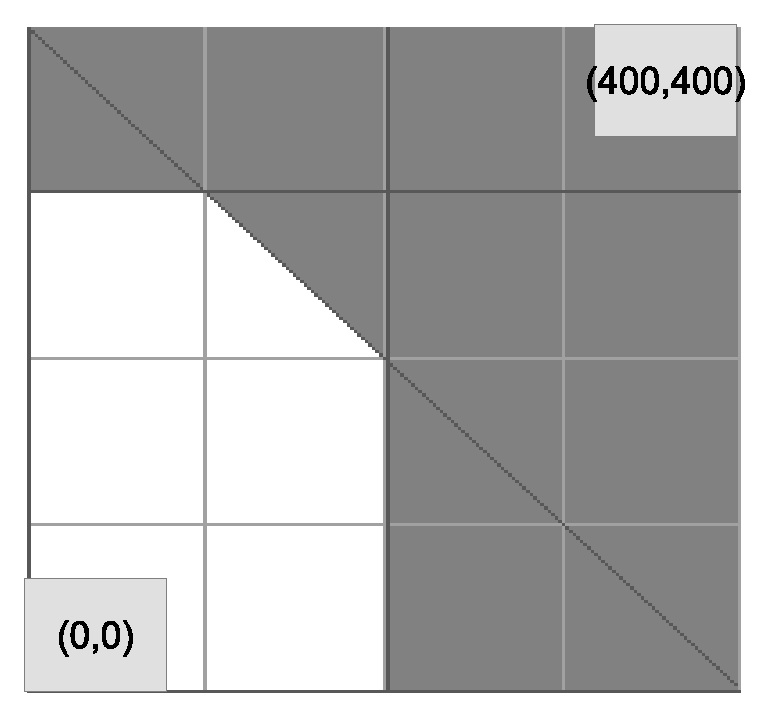
\includegraphics[width=2.0in]{figures/feasible-region}
\caption{\label{fig:feasible-region}Feasible-region in white (each unit 100)}
\end{center}
\end{figure}

Also we can convert the problem to another LP problem which aims to get the minimum result.
We can give coefficient $y_{1}$, $y_{2}$ and $y_{3}$ to the constraints 1, 2 and 3, and then sum them up. Then we can get:

($y_{1}$ + $y_{3}$)*$x_{1}$ + ($y_{2}$ + $y_{3}$)*$x_{2}$ $\le$ 200*$y_{1}$ + 300*$y_{2}$ + 400*$y_{3}$.

Let $y_{1}$ + $y_{3}$ = 1 and $y_{2}$ + $y_{3}$ = 6. As we want to maximize $x_{1}$ + 6$x_{2}$. We can convert it to the problem which minimize 200*$y_{1}$ + 300*$y_{2}$ + 400*$y_{3}$ with the constraints:
\begin{enumerate}
	\item $y_{1}$ + $y_{3}$ $\geq$ 1;
	\item $y_{2}$ + $y_{3}$ $\geq$ 6.
\end{enumerate}

So multiple 1 with 100 and 2 with 300, we can get

$x_{1}$ + 6$x_{2}$ $\le$ ($y_{1}$ + $y_{3}$)*$x_{1}$ + ($y_{2}$ + $y_{3}$)*$x_{2}$ $\le$ 200*$y_{1}$ + 300*$y_{2}$ + 400*$y_{3}$

$x_{1}$ + 6$x_{2}$ $\le$ 100*1 + 300*6 = 1900 which is the same as we get from the simplex algorithm.

\section{Primal-dual Method}
The convertion between maximum and minimum is called primal-dual.  Duality means that optimization problems may be viewed from either of two perspectives, the primal problem or the dual problem (the duality principle).  The solution to the dual problem provides a lower bound to the solution of the primal (minimization) problem.  Thus, a solution to the dual problem provides a bound on the value of the solution to the primal problem; when the problem is convex and satisfies a constraint qualification, then the value of an optimal solution of the primal problem is given by the dual problem.

Consider the general linear Programming 
\begin{enumerate}
	\item minimize $c^{T}x$
	\item subject to Ax ≥ b
	\item x ≥ 0 where $x = (x1, . . . , xn)^T$ is vector of variables, A = (Aij ) is an m × n matrix, and $c = (c1, . . . , cn)^T$ and $b = (b1, . . . , bm)^T$. Recall that the dual of this linear program is given by
	\item maximize $b^{T}y$
	\item subject to AT y ≤ c
	\item y ≥ 0 where $y = (y1, . . . , ym)^T$ is a vector of variables. The variables in y are in one-to-one correspondence with the constraints of the primal LP, and the variables in x are in one-to-one correspondence with
the constraints of the dual LP.
\end{enumerate}

\begin{theorem}
If an linear programming has a bounded optimal value, then so does its dual. And these optimal values are the same.
\end{theorem}

\end{document}
